\documentclass{article}
% General document formatting
\usepackage[margin=1.4in]{geometry}
\usepackage[parfill]{parskip}
\usepackage[utf8]{inputenc}
\usepackage{amssymb}
\usepackage[fleqn]{amsmath}
\usepackage{graphicx}
\usepackage{color}
\usepackage{amsthm}
% Related to math
\usepackage{amsmath,amssymb,amsfonts,amsthm}

\newtheorem{thm}{Theorem}

\title{Information Theory and Coding: Computer Assignment}
\author{Behrad Moniri (95109564)\\\texttt{bemoniri@live.com}}
\date{}
\begin{document}
	\maketitle
	\section{Estimating Mutual Information: Review}
	
	In this section, we will review  methods of estimating mutual information from finite samples and we will implement the KDR algorithm to estimate the mutual information and test the correctness of the algorithm in a simulation.
	\subsection{The Naive Approach: Binning and Histograms}
	The most naive method of estimating mutual information is by estimating a histogram and using the histogram for mutual information estimation. This method is know to be significantly biased.
	
	$$I(X, Y) \approx I_{\mathrm{binned}}(X, Y) = \sum_{i, j}^{} p(i, j) \log\Big(\frac{p(i, j)}{p_x(i) _y(j)}\Big)$$
	
	Here, $p_x$, $p_y$ and $p$ are estimations of the probability distribution function using histograms. Besides being biased, this method also is very dependent on the bin size \cite{cellucci2005statistical, wang2009universal}.
	
	\subsection{Adaptive Binning}
	This method is an extension of the naive method mentioned above. This method is widely used the signal processing literature for blind source separation. In contrast to the method described above, here the main idea is choose the bin size adaptability. The idea is to put more emphasis on areas with more variation in input space.

	Initially, we consider a one-cell partition involving all data pairs. In every iteration, cells are divided into equiprobable halves. The partitioning of each cell is accepted unless the ration $\frac{f_{XY}(x, y)}{f_X(x)f_Y(y)}$ takes approximately the same value in each of the four sub-cells as it does in the cell itself \cite{petr}.
	\begin{figure}[h!]
		\centering
		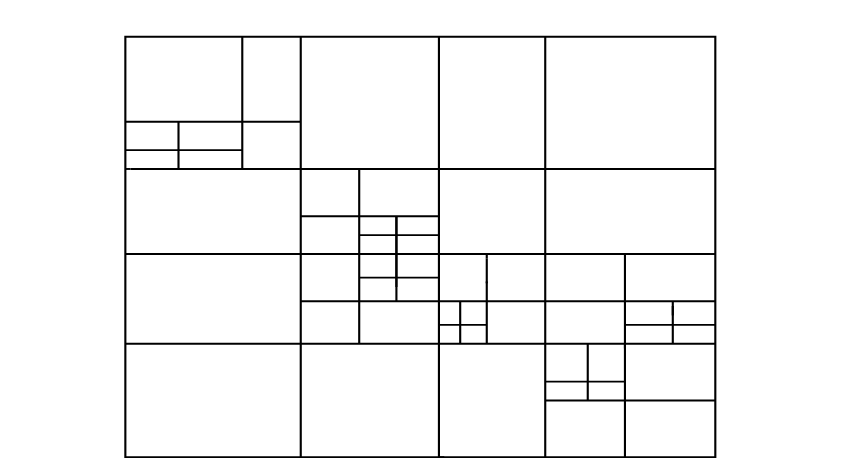
\includegraphics[scale = 0.35]{adaptive.png}
		\caption{Example of Adaptive Bin Size}
	\end{figure}

	\subsection{k Nearest Neighbor (kNN) Based Methods}
	
	Given  i.i.d. samples ${X_1,\dots,X_n}$ generated from density $p_X$, the problem is to estimate $p_X$ at  a  given  point $x_0$.  The k-NN of $x_0$ in ${X_1,...,X_n}$ is $X_{i(k)}$, where $i(1),\dots,i(n)$  is  such  that $||x_0-X_{i(1)}|| \leq ||x_0-X_{i(2)}|| \leq \dots \leq ||x_0-X_{i(n)}||$. Let $\rho_k$ be the distance between $x_0$ and the k-th  neighbor. The density $p_X$ can be estimated as:
	$$\hat{p}_X(x) = \frac{k(n)/n}{\lambda(B_{x, \rho_k})}$$
	
	Where $B_{x, \rho_k}$ is the ball centered at $x$ with radius $\rho$.
	\begin{thm}
		$$\lim_{n \to \infty} |\hat{p}_X(x) - p_X(x)| \to 0, \;\;\; \mathrm{almost\;\;surely}$$ provided $\frac{k(n)}{\log n} \to \infty$ and $\frac{n}{k(n)} \to \infty$.
	\end{thm}

	We will use the following notion of distance in the space $\mathbb{R}^{d_X + d_Y}$ i which $z = (x, y)$:
	$$||z-z'|| = \max\{||x-x'||, ||y-y'||\}$$
	
	Denote by $\epsilon(i)/2$ the distance from $z$ ito its k-NN, and by $\epsilon(x(i)/2)$ and $\epsilon (y(i)/2)$ the distances between the same points projected into the $X$ and $Y$ sub-spaces. $n_x(i)$ is the number of points whose distance from $x_i$ is strictly less than $\epsilon(i)/2$, andn $y(i)$ is similarly defined for $y$. The estimate for $I(X;Y)$ is
	$$I( X;Y) \approx -\frac{1}{n} \sum_{i = 1}{n} [\psi(n_x(i) + 1) + \psi(n_y(i) + 1)]  + \psi(k) + \psi(n)$$
	where $\psi$ is the Digamma function \cite{cellucci2005statistical}.
	
	\begin{figure}[h!]
		\centering
		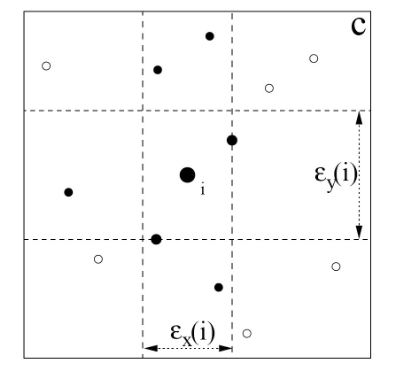
\includegraphics[scale=0.5]{knn.png}
		\caption{an example of kNN method with k = 1}
	\end{figure}
	
	\subsection{Kernel Density Estimation (KDE)}
	
	Another method for estimating mutual information is kernel density estimation. The density of a random variable (vector) $X$ can be estimated from i.i.d. samples, $X_1, X_2, \dots, X_n$ with the following equations:
	$$\hat{p}_X(z) = \frac{1}{n w_n^{d_X}} \sum_{i = 1}^{n} K\Big(\frac{z - X}{w_n}\Big)$$
	where $d_X$ is the dimension of $X$. $w_n$ controls the width  of the kernel and $w_n$ is a sequence convergent to zero. 
	
	Given this estimate, we can estimate the mutual information:
	
	$$\hat{I}(X;Y) = \frac{1}{n} \sum_{i = 1}^{n} \log \frac{\hat{p}_{XY}(X_i, Y_i)}{\hat{p}_X(X_i)\hat{p}_Y(Y_i)}$$
	
	This results are from \cite{wang2009universal}.
	
	\subsection{Choosing the algorithm to implement}
	I have been working on BSS and Sparse Recovery as my BSc thesis and I am familiar with estimators of mutual information. To my knowledge (gained over the time I worked on my BSc thesis), given a large sample size, the kernel estimation method gives the most accurate results for estimating mutual information. For this reason, we will implement this algorithm. The adaptive binning method is also very efficient and the time complexity is very low, but very good implementations of this algorithm already exist. We will use this algorithm (the implementation of adaptive binning algorithm is not done me!) to compare its results with the results of the algorithm I have implemented.

	
	\section{Implementation of KDE and Simulations}
	By comparing the simulation results of the mentioned methods in the literature, we decided to implement the KDE algorithm. We will use the gaussian kernel for estimation.
	
	The generative model of the data is:
	\begin{equation*}
	\begin{cases}
	X = N_1\\
	Y = X + N_2
	\end{cases}
	\end{equation*}
	where $N_1$ and $N_2$ are independent standard Gaussian random variables. In theory we know that the mutual information of two jointly Gaussian random variables is $-\frac{1}{2} \ln (1-\rho^2)$. The covariance matrix of our data is $\begin{bmatrix}
	15 & 15\\
	15 & 16
	\end{bmatrix}$, thus $I(X; Y) = 0.3466$. We will use a sample size of 1024 for estimation. Besides using our own implementation of KDE, we also use a well known implementation of the adaptive algorithm. . From theory we know that:
	$$I(X; Y) = \frac{1}{2} \log_2 (1 + \frac{P}{N})$$
	The results are presented in table \ref{resfig}. These results are from \cite{wang2009universal}.
	\begin{table}[h!]
		\centering
		\begin{tabular}{|c|c|c|}
			\hline
			Theory & KDE    & Adaptive \\ \hline
			2.000 & 2.5525 & 2.4302   \\ \hline
		\end{tabular}
	\caption{Simulation Results}
	\label{resfig}
	\end{table}
	
	
	\section{Estimating Channel Capacity and the Blahut-Arimoto Algorithm}
	
	In this section, we will implement the Blahut-Arimoto algorithm to estimate the channel capacity \cite{yeung2008blahut}. This algorithm is based on alternative optimization and update of the distribution and  an auxiliary variable. \textbf{I have read and understood the reasoning behind BL algorithm, but I will not repeat the theorems and results here, all can be found in \cite{yeung2008blahut}. I can explain this algorithms to the teaching assistants when requested!}
	
	
	
	The Blahut-Arimoto is presented below:
	
	\textbf{Init}: Initialize $p(1)$ to the uniform distribution over $\chi$, i.e. $p_i(1)=\frac{1}{|\chi|}$
	
	\textbf{Step 2}: Find $\phi^{(t+1)}$ as follows:
	$$\phi^{(t+1)} = \frac{p_i^{(t)} Q_{ij}}{\sum_{k}^{} p_k^{(t)} Q_{kj}}$$
	
	\textbf{Step 3}: Update $p^{(t+1)}$ as follows:
	$$p_i^{(t+1)} = \frac{r_i^{(t+1)}}{\sum_{k \in \chi}^{} r_k^{(t+1)}}$$
	
	\subsection{Experimental Results}
	\subsubsection{Channel A}
	
	In this channel the transition matrix is
	$$\begin{bmatrix}
	0.7&0.2&0.1\\
	0.1&0.2&0.7
	\end{bmatrix}$$
	
	The output of the BL algorithm  is: $\hat{C} =0.3651 $
	\subsubsection{Channel B}
	
	There must be a typo in the assignment. Rows of the transition matrix of this channel do not have unit sum.
	
	\subsubsection{Channel C}
	In this channel the transition matrix is
	$$\begin{bmatrix}
	0.7&0.3&0\\
	0&0.3&0.7
	\end{bmatrix}$$
	
		The output of the BL algorithm is: $\hat{C} =0.7000 $.
		This is correct as the channel is a BEC with error probability $0.3$, thus the capacity is $C = 0.7$.
		
		\bibliographystyle{unsrt}   % this means that the order of references
		% is dtermined by the order in which the
		% \cite and \nocite commands appear
		\bibliography{bib.bib}  % list here all the bibliographies that
		% you need. 
		
\end{document}